\documentclass[mathserif]{beamer}
\usetheme{singapore}
\usepackage{graphicx}
\usepackage{tabularx}
\usepackage{longtable}
\usepackage{multicol}
\usepackage{epstopdf}
\usepackage{amssymb}
\title{Skills, Tasks and Technologies: Implications for Employment and Earnings}
\author{Daron Acemoglu and David Autor}
\institute{Handbook of Labour Economics, Volume 4b, 2011}
\date{17th October 2014}
\begin{document}
\frame{\titlepage}
\begin{frame}
\frametitle{Key aim of the paper:}
\begin{center}
To introduce a rich theoretical framework to explain the recent changes in earnings and employment distribution in advanced economies - The Ricardian model
\end{center}
\end{frame}
\AtBeginSection[]
{
  \begin{frame}
    \frametitle{Table of Contents}
    \tableofcontents[currentsection]
  \end{frame}
}
\section{Recent trends in the labour market}
\begin{frame}
\frametitle{Increase in college wage premium}
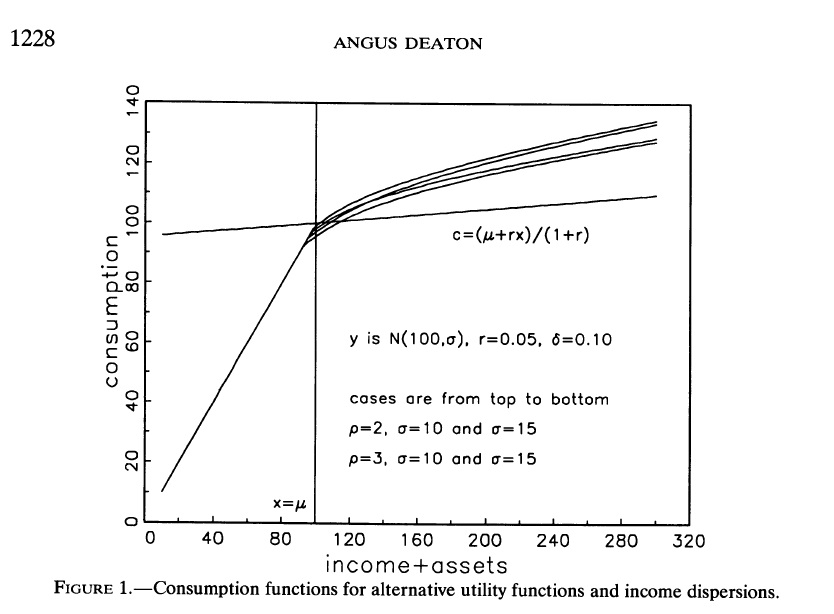
\includegraphics[scale=0.5]{figure1}
\end{frame}
\begin{frame}
\frametitle{Despite increase in supply of college graduates}
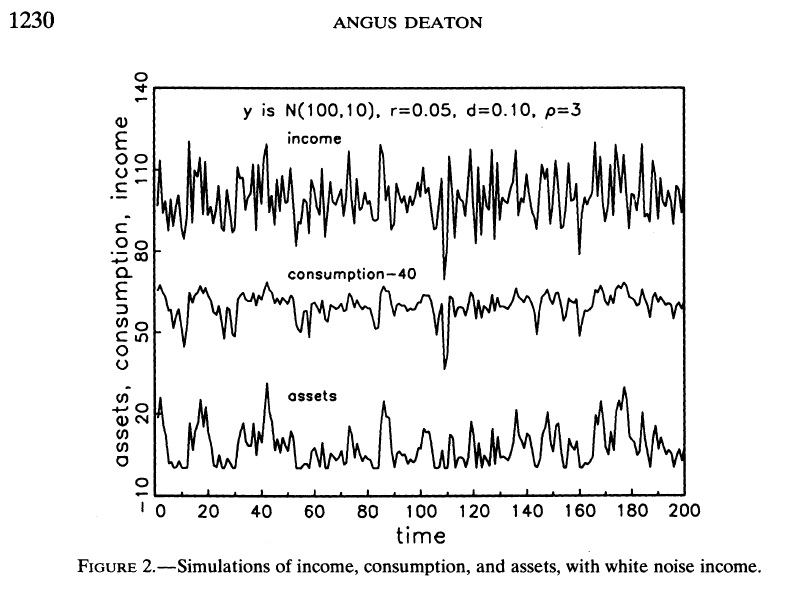
\includegraphics[scale=0.5]{figure2}
\end{frame}
\begin{frame}
\frametitle{Decline in real wages of low skill workers}
\includegraphics[scale=0.5]{figure4a}
\end{frame}
\begin{frame}
\frametitle{Decline in real wages of low skill workers}
\includegraphics[scale=0.5]{figure4b}
\end{frame}
\begin{frame}
\frametitle{Wage polarization}
\includegraphics[scale=0.5]{figure9b}
\end{frame}
\begin{frame}
\frametitle{Wage polarization}
\includegraphics[scale=0.5]{figure9c}
\end{frame}
\begin{frame}
 \frametitle{Non-monotone shift in the composition of employment across occupations}
\includegraphics[scale=0.4]{figure10}
\end{frame}
\begin{frame}
\frametitle{Accompanied by changes in the allocation of skills across occupations}
\includegraphics[scale=0.4]{figure14a}
\end{frame}
\begin{frame}
\frametitle{Accompanied by changes in the allocation of skills across occupations}
\includegraphics[scale=0.5]{figure14b}
\end{frame}
\begin{frame}
\frametitle{Recent technological changes and trends in offshoring directly replacing routine task workers}
\begin{itemize}
\item \textit{The job routinization hypothesis}: job polarization is due to rising productivity and declining real price of ICT, which is used to perform routine tasks.
\item Routine task: A procedural, rule-based task to which computers are well-suited. Characteristic of many middle-skill jobs, eg. clerical work and administrative occupations
\item ICT advances have also lowered the cost of offshoring
\end{itemize}
\end{frame}
\section{The Canonical Model and its shortcomings}
\begin{frame}
\frametitle{The Canonical Model in three slides}
\begin{itemize}
\item Two types of workers (exogenously given): high and low skill, no distinction between skills and tasks
\item High skill and low skill workers perform different tasks and are imperfect substitutes
\begin{equation*}
Y=[(A_LL)^\frac{\sigma-1}{\sigma}+(A_HH)^\frac{\sigma-1}{\sigma}]^\frac{\sigma}{\sigma-1}
\end{equation*}
Where $\sigma$ is the elasticity of substitution between high and low skill labour, and $A_L$ and $A_H$ are factor-augmenting technology terms.
\item Labour markets are competitive, each type of worker paid their marginal productivity.
\end{itemize}
\end{frame}
\begin{frame}
\frametitle{The Canonical Model in three slides}
\begin{equation*}
w_L=\frac{\delta Y}{\delta L}=A_L^{\frac{\sigma-1}{\sigma}}[A_L^{\frac{\sigma-1}{\sigma}}+A_H^{\frac{\sigma-1}{\sigma}}(H/L)^{\frac{\sigma-1}{\sigma}}]^\frac{1}{\sigma-1}
\end{equation*}
\begin{itemize}
\item Note $\frac{\delta w_L}{\delta (H/L)}>0$ because high skill and low skill workers are imperfect substitutes, $\frac{\delta w_L}{\delta A_L}>0$  and $\frac{\delta w_L}{\delta A_H}>0$.
\begin{equation*}
w_H=\frac{\delta Y}{\delta H}=A_H^\frac{\sigma-1}{\sigma}[A_L^\frac{\sigma-1}{\sigma}(H/L)^{-\frac{\sigma-1}{\sigma}}+A_H^\frac{\sigma-1}{\sigma}]^\frac{1}{\sigma-1}
\end{equation*}
\item Note $\frac{\delta w_H}{\delta (H/L)}<0$, $\frac{\delta w_H}{\delta A_L}>0$ and $\frac{\delta w_H}{\delta A_H}>0$.
\item An improvement in any one of the factor augmenting technologies should increase wages of both groups.
\end{itemize}
\end{frame}
\begin{frame}
\frametitle{The Canonical Model in three slides}
\begin{itemize}
\item The skills premium can be expressed as
\begin{equation*}
\omega=\frac{w_H}{w_L}=(\frac{A_H}{A_L})^\frac{\sigma-1}{\sigma}(\frac{H}{L})^\frac{-1}{\sigma}
\end{equation*}
\item Taking logs,
\begin{equation*}
ln\omega=\frac{\sigma-1}{\sigma}ln(\frac{A_H}{A_L})-\frac{1}{\sigma}ln(\frac{H}{L})
\end{equation*}
\item Note $\frac{\delta ln\omega}{\delta lnH/L}=-\frac{1}{\sigma}$ and $\frac{\delta ln\omega}{\delta ln(A_H/A_L)}=\frac{\sigma-1}{\sigma}$. Empirically, $\sigma>1$.
\item Empirically $H/L$ has increased over time. $\frac{A_H}{A_L}$ must have increased since college skills premium has been rising.
\end{itemize}
\end{frame}
\begin{frame}
\frametitle{Main problems of Canonical Model}
\begin{itemize}
\item No explanation for why some workers (less-educated workers) have experienced real earnings declines in the last three decades
\item No framework to understand wage polarization
\item No distinction between skills and tasks - cannot account for why allocation of skill groups across occupations has shifted (more middle educated in low education service jobs)
\item No framework to study how technologies (or offshoring) can displace some workers from their jobs
\item Technical change treated as exogenous
\end{itemize}
\end{frame}
\section{A Ricardian Model of the Labour Market}
\begin{frame}
\frametitle{A Ricardian Model of the Labour Market - setup}
\begin{itemize}
\item Model based on Acemoglu and Zilibotti (2001)
\item A \textit{task}: a unit of work activity that produces output
\item A \textit{skill}: an endowment of capabilities for performing various tasks
\item Skills are applied to tasks to produce output. With a given skill level, a worker can perform a variety of tasks
\item Key role played by CA differences between workers
\item Low-skill tasks$\approx$ manual and service occupations, medium-skill tasks $\approx$ sales, clerical and adminstrative support occupations (routine), high-skill tasks $\approx$ managerial, professional and technical occupations (abstract)
\end{itemize}
\end{frame}
\begin{frame}
\frametitle{The environment}
\begin{itemize}
\item Static environment, closed economy
\item Unique final good (numeraire) produced by a continuum of tasks
\begin{equation*}
Y=exp[\int_0^1lny(i)di]
\end{equation*}
Where $Y$ is the output of the unique final good, $y(i)$ is the production level of task $i$.
\item All markets are competitive
\item Fixed inelastic total supply of high (H), medium (M) and low (L) skilled workers. These are (for now) the three FOPs.
\item Assume no capital for now
\end{itemize}
\end{frame}
\begin{frame}
\frametitle{The environment - baseline model}
\begin{itemize}
\item The production of each task $i$ is
\begin{equation*}
y(i)=A_L\alpha_L(i)l(i)+A_M\alpha_M(i)m(i)+A_H\alpha_H(i)h(i)
\end{equation*}
\item $A_L$, $A_M$, $A_H$ - low skill biased tech,  medium skill biased tech,  high skill biased tech respectively
\item $\alpha_L(i)$,$\alpha_M(i)$,$\alpha_H(i)$ - productivity of low skill, medium skill, high skill workers in task $i$ respectively
\item $l(i)$,$m(i)$,$h(i)$ - the number of low skill, medium skill and high skill workers involved in producing task $i$
\item Each task can be performed by a worker of any skill, but each skill group has different CAs over each task, depending on $\alpha$s.
\end{itemize}
\end{frame}
\begin{frame}
\frametitle{The environment - baseline model}
\begin{itemize}
\item \textbf{Assumption 1}: $\frac{\alpha_L(i)}{\alpha_M(i)}$ and $\frac{\alpha_M(i)}{\alpha_H(i)}$ are continuously differentiable and strictly decreasing in $i$.
\item The complexity of the task is increasing in index $i$.
\item Factor market clearing requires
\begin{equation*}
\int_0^1l(i)di\leq L \quad \int_0^1m(i)di\leq M \quad \int_0^1h(i)di\leq H
\end{equation*}
\end{itemize}
\end{frame}
\begin{frame}
\frametitle{The equilibrium - Allocation of skills of tasks}
The equilibrium is an allocation in which producers maxmize profits and labour markets clear
\begin{itemize}
\item Two thresholds exist in equilibrium: $I_L$ and $I_H$
\item \textbf{Lemma 1}: In any equilibrium there exist $I_L$ and $I_H$ such that $0<I_L<I_H<1$ for any $i<I_L$, $m(i)=h(i)=0$, for any $i\in (I_L,I_H)$, $l(i)=h(i)=0$, and for any $i>I_H$, $l(i)=m(i)=0$.
\item The set of tasks will be partitioned into three sets, separated by thresholds $I_L$ and $I_H$.
\item $I_L$ and $I_H$ are endogenous and will respond to changes in skill supplies and technology
\end{itemize}
\end{frame}
\begin{frame}
\frametitle{The equilibrium - The law of one price of skills}
Though workers of the \textit{same skill level} perform different tasks, they receive the \textit{same} wage.
\begin{itemize}
\item Let $p(i)$ be the price of the task $i$. Setting the price of the final good to one,
\begin{equation*}
exp[\int_0^1lnp(i)di]=1
\end{equation*}
\item In equilibrium, all workers within each skill category must be paid the same wage, regardless of the tasks they perform. Hence
\begin{multline*}
w_L=p(i)A_L\alpha_L(i) \quad \text{for any} i<I_L
\\ w_M=p(i)A_M\alpha_m(i) \quad \text{for any} I_L<i<I_H
\\ w_H=p(i)A_H\alpha_H(i) \quad \text{for any} i>I_H
\end{multline*}
\end{itemize}
\end{frame}
\begin{frame}
\frametitle{The equilibrium - The law of one price of skills}
The productivity difference of a given type of worker in two different tasks must be exactly offset by the price difference between these two tasks. I.e.
\begin{multline*}
p(i)\alpha_L(i)=p(i')\alpha_L(i')\equiv P_L \quad \text{for any} i,i'<I_L
\\ p(i)\alpha_M(i)=p(i')\alpha_M(i')\equiv P_M \quad \text{for any} I_H>i,i'>I_L
\\ p(i)\alpha_H(i)=p(i')\alpha_H(i')\equiv P_H \quad \text{for any} i,i'>I_H
\end{multline*}
Where $P_L$, $P_M$ and $P_H$ are the price indexes of tasks performed by low, medium and high skill workers respectively.
\end{frame}
\begin{frame}
\frametitle{The equilibrium - How many workers perform each task?}
\begin{itemize}
\item Cost minimization in the production of final good gives $p(i)y(i)=p(i')y(i')$ for any $i,i'$.
\item Considering two tasks $i,i'<I_L$ performed by low skill workers, $p(i)\alpha_L(i)l(i)=p(i')\alpha_L(i')l(i')$ holds.
\item Since $p(i)\alpha_L(i)=p(i')\alpha_L(i')\equiv P_L$, it must be that $l(i)=l(i')$. With the market clearing condition for low skill workers
\begin{equation*}
l(i)=\frac{L}{I_L} \quad for \quad i<I_L
\end{equation*}
\item By a smiliar logic,
\begin{multline*}
m(i)=\frac{M}{I_H-I_L} \quad for \quad I_H>i>I_L
\\ h(i)\frac{H}{1-I_H} \quad for \quad i>I_H
\end{multline*}
\end{itemize}
\end{frame}
\begin{frame}
\frametitle{The equilibrium - Relative price index for tasks performed by different skill groups}
\begin{itemize}
\item Comparing two tasks performed by high and medium skill workers, and the same for two tasks performed by medium and low skill workers,
\begin{multline*}
p(i)A_M\alpha_M(i)m(i)=p(i')A_H\alpha_H(i')h(i') \quad \text{for} \quad I_L<i<I_H<i'
\\ p(i)A_L\alpha_L(i)l(i)=p(i')A_M\alpha_M(i')m(i') \quad \text{for} \quad i<I_L<i'<I_H
\end{multline*}
\item After some manipulation, they obtain
\begin{equation*}
\frac{P_H}{P_M}=(\frac{A_HH}{1-I_H})^{-1}(\frac{A_MM}{I_H-I_L}), \quad
\frac{P_M}{P_L}=(\frac{A_MM}{I_H-I_L})^{-1}(\frac{A_LL}{I_L})
\end{equation*}
\end{itemize}
\end{frame}
\begin{frame}
\frametitle{The equilibrium - No arbitrage across skills}
\begin{itemize}
\item Key equilibrium objects $I_H$ and $I_L$ are determined by two no arbitrage conditions.
\item  Equilibrium supply of task $I_H$ should be the same whether produced by high or medium skill worker. Same reasoning for task $I_L$. This gives
\begin{multline*}
y(I_H)=\alpha_H(I_H)A_Hh(I_H)=\alpha_M(I_H)A_Mm(I_H)
\\ y(I_L)=\alpha_L(I_L)A_Ll(I_L)=\alpha_M(I_L)A_Mm(I_L)
\end{multline*}
Which gives
\begin{multline*}
\frac{A_M\alpha_M(I_H)M}{I_H-I_L}=\frac{A_H\alpha_H(I_H)H}{1-I_H}
\\ \frac{A_L\alpha_L(I_L)L}{I_L}=\frac{A_M\alpha_M(I_L)M}{I_H-I_L}
\end{multline*}
\end{itemize}
\end{frame}
\begin{frame}
\frametitle{The equilibrium - Equilibrium wages and inequality}
\begin{itemize}
\item Using expressions $\frac{P_H}{P_M}$ and $\frac{P_M}{P_L}$, they obtain the ratio of wages across skill groups in terms of thresholds and skill supplies
\begin{multline*}
\frac{w_H}{w_M}=(\frac{1-I_H}{I_H-I_L})(\frac{H}{M})^{-1}
\\ \frac{w_M}{w_L}=(\frac{I_H-I_L}{I_L})(\frac{M}{L})^{-1}
\end{multline*}
\item Using $\int_0^1lnp(i)di=0$ and the law of one price for skills equations we get the last equilibrium condition
\begin{multline*}
\int_0^{I_L}(lnP_L-ln\alpha_L(i))di+\int_{I_L}^{I_H}(lnP_M-ln\alpha_M(i))di \\ +\int_{I_H}^1(lnP_H-ln\alpha_H(i))di=0
\end{multline*}
\end{itemize}
\end{frame}
\begin{frame}
\frametitle{The equilibrium - Summary of equilibrium}
\textbf{Proposition 1}: There exits a unique equilibrium summarized by $(I_L,I_H,P_L,P_M,P_H,w_L,w_M,w_H)$. With the 2 no arbitrage conditions,
\includegraphics[scale=0.5]{figure22}
\end{frame}
\begin{frame}
\frametitle{The equilibrium - Summary of equilibrium}
Rewriting the two no arbitrage conditions, they obtain:
\begin{equation*}
\underbrace{\frac{1-I_H}{I_H-I_L}\frac{\alpha_M(I_H)}{\alpha_H(I_H)}}_{\text{Relative effective dd of h to m skills}}=\overbrace{\frac{A_HH}{A_MM}}^{\text{Relative effective ss of h to m skills}}
\end{equation*}
\begin{equation*}
\underbrace{\frac{I_H-I_L}{I_L}\frac{\alpha_L(I_H)}{\alpha_M(I_H)}}_{\text{Relative effective dd of m to l skills}}=\overbrace{\frac{A_MM}{A_LL}}^{\text{Relative effective ss of m to l skills}}
\end{equation*}
\end{frame}
\begin{frame}
\frametitle{The equilibrium - Summary of equilibrium}
\includegraphics[scale=0.5]{figure23}
\end{frame}
\section{Comparative statics of the Ricardian model}
\begin{frame}
\frametitle{Comparative statics}
\begin{itemize}
\item To study comparative statics, take logs of the no arbitrage conditions
\begin{equation*}
lnA_M-lnA_H+\beta_H(I_H)+ln_M-ln_H-ln(I_H-I_L)+ln(1-I_H)=0
\end{equation*}
\begin{equation*}
lnA_L-lnA_M+\beta_L(I_L)+lnL-ln_M+ln(I_H-I_L)-ln(I_L)=0
\end{equation*}
Where $\beta_H(I)\equiv ln\alpha_M(I)-ln\alpha_H(I)$ and $\beta_L(I)\equiv ln\alpha_L(I)-ln\alpha_M(I)$.
\end{itemize}
\end{frame}
\begin{frame}
\frametitle{Comparative statics}
\textbf{Proposition 2} The following comparative static results apply \\
\textit{1. The response of task allocation to technology and skill supplies}:
\begin{multline*}
\frac{dI_H}{dlnA_H}=\frac{dI_H}{dlnH}<0, \quad \frac{dI_L}{dlnA_H}=\frac{dI_L}{dlnH}<0, \\ \frac{d(I_H-I_L)}{dlnA_H}=\frac{d(I_H-I_L)}{dlnH}<0
\end{multline*}
Increase in $A_H$ and $H$ expands set of tasks performed by high skill workers, reduces sets of tasks performed by middle skill (direct effect) and low skill (indirect effect) workers.
\end{frame}
\begin{frame}
\frametitle{Comparative statics}
\includegraphics[scale=0.5]{figure26}
\end{frame}
\begin{frame}
\frametitle{Comparative statics - \textbf{Proposition 2} continued}
\textit{2. The response of relative wages to skill supply changes}
\begin{equation*}
\frac{dln(w_H/w_L)}{dlnH}<0, \quad \frac{dln(w_H/w_M)}{dlnH}<0
\end{equation*}
Increase in supply of high skill workers, all else equal, lowers high skill worker wages relative to low skill and middle skill worker wages
\end{frame}
\begin{frame}
\frametitle{Comparative statics - \textbf{Proposition 2} continued}
\textit{3. The response of wages to factor-augmenting technologies}
\begin{equation*}
\frac{dln(w_H/w_L)}{dlnA_H}>0, \quad \frac{dln(w_M/w_L)}{dlnA_H}<0, \quad \frac{dln(w_H/w_M)}{dlnA_H}>0
\end{equation*}
\begin{itemize}
\item Increase in $A_H$ increases the wage of the high skill worker relative to the low and medium skill worker, and decreases the wage of the middle skill worker relative to the low skill worker (indirect vs direct effect) - The U shape
\item Authors show, with some specifications for $\alpha(i)$s that an increase in $lnA_H$ can lower $lnP_M$ and hence $w_M$ $\rightarrow$ A factor augmenting increase in productivity for high skill workers can also lower the \textit{level} of wages for lower skill groups by \textit{shrinking the set of tasks they can perform}.
\end{itemize}
\end{frame}
\begin{frame}
\frametitle{What happens if machines, which displace some workers from their tasks, are introduced?}
\begin{itemize}
\item  Routine tasks are most likely to be displaced by recently invented machines
\item Routine tasks primarily performed by middle-skilled workers
\item Assume now a range of tasks $[I',I'']\subset [I_L,I_H]$ that are more economically performed by machines than medium-skilled workers.
\end{itemize}
\end{frame}
\begin{frame}
\frametitle{What happens if machines, which displace some workers from their tasks, are introduced?}
\textbf{Proposition 3}: After the introduction of machines, there exist new equilibrium thresholds $\hat{I}_L$ and $\hat{I}_H$ such that $0<\hat{I}_L<I'<I''<\hat{I}_H<1$ and for any $i<\hat{I}_L$, $m(i)=h(i)=0$ and $l(i)=L/\hat{I}_L$; for any $i\in (\hat{I}_L,I')\cup(I'',\hat{I}_H)$, $l(i)=h(i)=0$ and $m(i)=M/(\hat{I}_H-I''+I'-\hat{I}_L)$; for any $i\in(I',I'')$, $l(i)=m(i)=h(i)=0$; and for any $i>\hat{I}_H$, $l(i)=m(i)=0$ and $h(i)=H/(1-\hat{I}_H)$.
\begin{itemize}
\item Letting $\epsilon$ be the length of the interval $[I',I'']$, they show that $\frac{dI_H}{d\epsilon}>0$, $\frac{dI_L}{d\epsilon}<0$ and $\frac{d(I_H-I_L)}{d\epsilon}>0$.
\item Reallocation of tasks in the economy - Medium skill workers perform some of tasks previously allocated to low-skill workers and to to high-skilled workers.
\end{itemize}
\end{frame}
\begin{frame}
\frametitle{What happens if machines, which displace some workers from their tasks, are introduced?}
\textbf{Proposition 4} Suppose we start with an equilibrium characterized by thresholds $[I_L,I_H]$ and technical change implies that the tasks in the range $[I',I'']\subset[I_L,I_H]$ are now performed by machines. Then:
\begin{enumerate}
\item $w_H/w_M$ increases
\item $w_M/w_L$ decreases
\item $w_H/w_L$ increases if $|\beta_L'(I_L)I_L|<|\beta_H'(I_H)(1-I_H)|$ and decreases if $|\beta_L'(I_L)I_L|> |\beta_H'(I_H)(1-I_H)|$
\end{enumerate}
Likely that $|\beta_L'(I_L)|<|\beta_H'(I_H)|$ $\rightarrow$  CA of high skill workers over medium skill workers in $I_H$ task $>$ CA of low skill workers over medium skill workers in $I_L$ task. I.e. Medium skill workers closer substitutes for low than high skill workers.
\end{frame}
\begin{frame}
\frametitle{Interpretation of US wage and employment structure through this framework}
\begin{itemize}
\item 1980s: Declining wages at the bottom of wage distribution and relative contraction in employment in low-wage occupations, as well as rising wages and employment in high skill occupations - due to increase in $A_H/A_M$ and $A_M/A_L$.
\item 1990s: U-shaped change in employment and wage percentiles - IT replaces middle skill tasks
\item 2000s: Employment in low skill service occupations grows more rapidly - due to movement of displaced medium skill workers into low skill jobs as $|\beta_L'(I_L)|<|\beta_H'(I_H)|$
\end{itemize}
\end{frame}
\section{Conclusion}
\begin{frame}
\frametitle{Conclusion}
\begin{itemize}
\item Ricardian model offers some explanations for recent labour market trends, performs better than Canonical model
\item \textbf{Other extensions by authors}: a) Endogenous choice of skill supply, b) Directed technical change
\item \textbf{Interesting extension by Lindenlaub (2013)}: Sorting of skills to jobs  with two skill dimensions - cognitive and manual.
\item \textbf{Limitations of model}: Competitive markets assumption, skill endowment assumed exogenous, unidimensional skills
\end{itemize}
\end{frame}
\end{document}
